\begin{figure}[h] 
\centering 
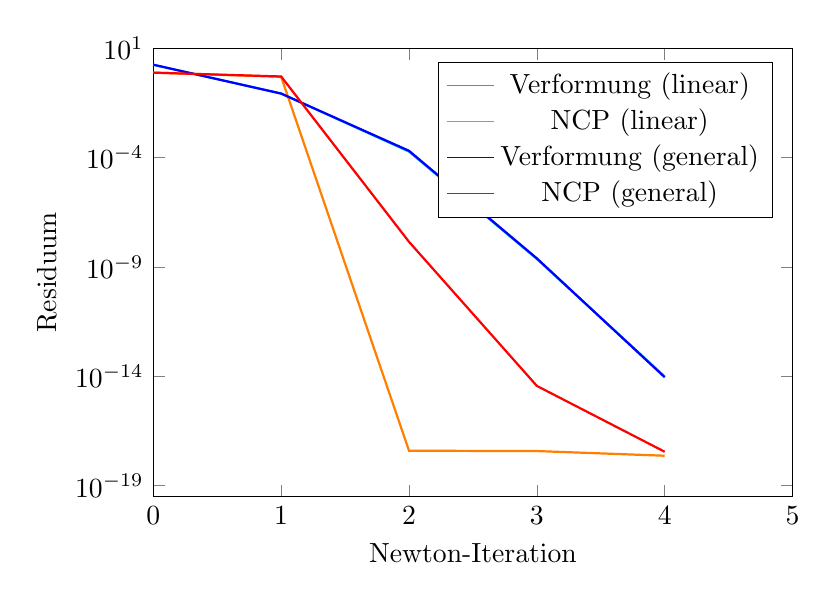
\begin{tikzpicture}[every plot/.append style={thick}] 
\begin{axis}[ 
label style={font=\normalsize}, 
xlabel={Newton-Iteration}, 
ylabel={Residuum}, 
xmin=0, xmax=5, 
ymode=log, 
ymin=0, ymax=10, 
width=0.8\textwidth, 
height=0.6\textwidth, 
legend pos=north east, 
legend style={cells={align=left}}, 
grid style=dashed, 
] 
\addplot[ 
color=cyan, 
] 
coordinates { 
(0, 1.75e+00)(1, 8.45e-02)(2, 1.88e-04)(3, 2.32e-09)(4, 9.85e-15)}; 
\addlegendentry{Verformung (linear)} 
\addplot[ 
color=orange, 
] 
coordinates { 
(0, 7.64e-01)(1, 4.91e-01)(2, 3.99e-18)(3, 3.86e-18)(4, 2.36e-18)}; 
\addlegendentry{NCP (linear)} 
\addplot[ 
color=blue, 
] 
coordinates { 
(0, 1.75e+00)(1, 8.39e-02)(2, 2.04e-04)(3, 2.47e-09)(4, 9.11e-15)}; 
\addlegendentry{Verformung (general)} 
\addplot[ 
color=red, 
] 
coordinates { 
(0, 7.60e-01)(1, 5.07e-01)(2, 1.41e-08)(3, 3.66e-15)(4, 3.58e-18)}; 
\addlegendentry{NCP (general)} 
\end{axis} 
\end{tikzpicture} 
\caption{Residuen des Stoffgesetzes 'Neo Hooke' mit Hinderniss 'Parabel' und 578 Freiheitsgraden für die Verschiebung.} 
\label{fiq:NeoHooke_Parabel_level3} 
\end{figure} 
